\section{The coupling method}

\indent We will explain in this section the scheme we propose for coupling the NSWE and the Serre equations. Without loss of generality, we will consider the domain $\Omega = \mathbb{R}$, divided in two subdomains $\Omega_1$ and $\Omega_2$, with $\Gamma = \Omega_1 \cap \Omega_2$, and we describe the conditions imposed on the interface $\Gamma$. We suppose that the Serre equations describe the wave propagation in $\Omega_1$, while the NSWE describe it in $\Omega_2$.

\subsection{The models}

\indent The NSWE and the Serre equations are given respectively by

\begin{equation}
\label{eq:nswe}
\begin{cases}
h_t + \left(hu\right)_x = 0 \\
u_t + uu_x + gh_x = 0
\end{cases}
\end{equation}

\begin{equation}
\label{eq:SerreFull}
\begin{cases}
h_t + (hu)_x = 0 \\
u_t + uu_x + gh_x - \frac{1}{3h}\left(h^3 \left( u_{xt} + uu_{xx} - (u_x)^2  \right) \right)_x = 0
\end{cases}
\end{equation}

\indent The main idea for the construction of our scheme is that the Serre equations \eqref{eq:SerreFull} are solved using a splitting method, which separates the advection terms from the dispersive ones. Therefore, the resolution of the Serre equations consists in solving, in each time step: 

\begin{equation}
\label{eq:SerreSplit1}
\begin{cases}
\th_t + \left(\th\tu\right)_x = 0 \\
\tu_t + \tu\tu_x + g\th_x = 0, \ \, t \in [t_n, t_{n+1}], \ \  (\th,\tu)(x,t_n) = (h,u)(x,t_n)
\end{cases}
\end{equation}

\begin{equation}
\label{eq:SerreSplit2}
\begin{cases}
\lh_t   = 0 \\
\lu_t - \frac{1}{3\lh}\left(\lh^3 \left( \lu_{xt} + \lu\lu_{xx} - (\lu_x)^2  \right) \right)_x = 0, \ \, t \in [t_n, t_{n+1}], \ \  (\lh,\lu)(x,t_n) = (\th,\tu)(x,t_{n+1})
\end{cases}
\end{equation}

\begin{equation}
\begin{cases}
(h,u)(x,t_{n+1}) = (\lh,\lu)(x,t_{n+1})
\end{cases}
\end{equation}

\indent If we denote the two systems by the operators $T_a^{\Delta t}$ and $T_d^{\Delta t}$, respectively, where the superscript indicates that the operator is performed over a time step $\Delta t$, the resolution of the Serre equations can be written as

\begin{equation}
(h,u)(x,t_{n+1}) = T_d^{\Delta t} \left( T_a^{\Delta t} \left((h,u)(x,t_n) \right) \right)
\end{equation}

\indent We remark that the first step of the splitted Serre equations (equation \ref{eq:SerreSplit1}) corresponds to the NSWE (equation \ref{eq:nswe}).

\indent Different numerical schemes are proposed for solving each one of these equations, taking advantage of their properties. The advection equation \eqref{eq:SerreSplit1} (and \ref{eq:nswe}), which can be written in a conservative form, is solved using a finite volume method, with an approximate Riemann solver and fourth-order MUSCL interpolation on each cell interface. The dispersive equation \eqref{eq:SerreSplit2} is solved using an explicit finite difference scheme with fourth-order spatial discretization. We refer to the previous reports for details about these implementations.

\subsection{The coupling}

\indent Our coupling scheme takes advantage of the fact that the first step of the splitted Serre equations is identical to the NSWE. Indeed we propose, in each time step :

\begin{enumerate}
	\item A Domain Decomposition Method between NSWE in $\Omega_1$ and NSWE in $\Omega_2$ (coupling between \eqref{eq:nswe} and \eqref{eq:SerreSplit1});
	\item A ``Domain Decomposition Method’’ between the dispersive equation \eqref{eq:SerreSplit2} in $\Omega_1$ and a zero solution in $\Omega_2$.
\end{enumerate}

\indent The quotes in the second step refer to the fact that a DDM between an equation and a zero solution is, in fact, a Transparent Boundary Condition problem.

\subsubsection{The interface conditions}

\indent Appropriate interface conditions must be imposed in order to the DDM problem give ``correct’’ solutions regarding the solution given by the monodomain problem. Before detailing the conditions imposed in each step of the coupling, we describe the spatial discretization around the interface.

\indent We define $\Omega_1$ and $\Omega_2$ such that they have exactly one common point, located on the interface $\Gamma$. Moreover, as the fourth-order finite volume scheme requires three ghost cells in each boundary, we extend the subdomains by three cells in each side, giving the discretization showed in the figure \ref{fig:discretization} : 

\indent

\begingroup
\centering
\tikzstyle{label} =[above,font=\tiny]
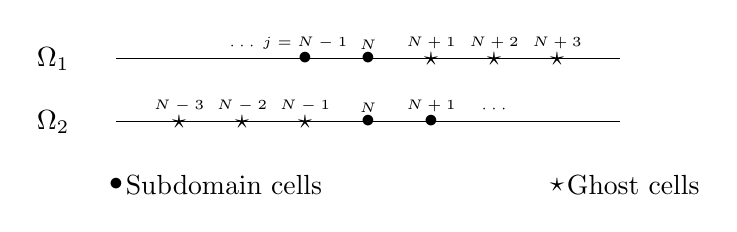
\begin{tikzpicture}[scale = .8]
	\coordinate (Alabel) at (-1,3);
	\coordinate (Aa) at (0,3);
	\coordinate (Ab) at (1,3);
	\coordinate (Ac) at (2,3);
	\coordinate (Ad) at (3,3);	
	\coordinate (Ae) at (4,3);	
	\coordinate (Af) at (5,3);	
	\coordinate (Ag) at (6,3);
	\coordinate (Ah) at (7,3);	
	\coordinate (Ai) at (8,3);	

	
	\draw (Aa) -- (Ai);
	\draw (Alabel) node {$\Omega_1$}; 
	\draw (Ac) node[label] {$\cdots$};
	\draw (Ad) node[label] {$j=N-1$};
	\draw (Ae) node[label] {$N$};
	\draw (Af) node[label] {$N+1$};
	\draw (Ag) node[label] {$N+2$};
	\draw (Ah) node[label] {$N+3$};
		
	\draw (Ad) node {$\bullet$};
	\draw (Ae) node {$\bullet$};
	\draw (Af) node {$\star$};
	\draw (Ag) node {$\star$};
	\draw (Ah) node {$\star$};
	
	\coordinate (Blabel) at (-1,2);	
	\coordinate (Ba) at (0,2);
	\coordinate (Bb) at (1,2);
	\coordinate (Bc) at (2,2);
	\coordinate (Bd) at (3,2);	
	\coordinate (Be) at (4,2);	
	\coordinate (Bf) at (5,2);
	\coordinate (Bg) at (6,2);	
	\coordinate (Bh) at (7,2);
	\coordinate (Bi) at (8,2);	

	\draw (Ba) -- (Bi); 
	\draw (Bb) node[label] {$N-3$};
	\draw (Bc) node[label] {$N-2$};
	\draw (Bd) node[label] {$N-1$};
	\draw (Be) node[label] {$N$};
	\draw (Bf) node[label] {$N+1$};
	\draw (Bg) node[label] {$\cdots$};
	
	\draw (Blabel) node {$\Omega_2$}; 
	\draw (Bb) node {$\star$};
	\draw (Bc) node {$\star$};	
	\draw (Bd) node {$\star$};
	\draw (Be) node {$\bullet$};	
	\draw (Bf) node {$\bullet$};
	
	
	%% Legend
	\draw (0,1) node {$\bullet$} node[right] {Subdomain cells};
	\draw (7,1) node {$\star$} node[right]  {Ghost cells};
	
\end{tikzpicture}
\captionof{figure}{Scheme indicating the spatial discretization of the subdomains around the interface  \label{fig:discretization}}
\endgroup 

\indent We remark that the solution is computed only in the  ``subdomain cells’’.

\subsubsection{Notation}

\indent The discrete solutions of the problem will be denoted as

\begin{equation*}
	\begin{gathered}
		u^{i,n}_{j,A}, \qquad u^{i,n}_{j,D} \qquad u^{i,n}_{j}  \\
		h^{i,n}_{j,A}; \qquad h^{i,n}_{j,D} \qquad h^{i,n}_{j}
	\end{gathered}
\end{equation*}

\noindent where $i$ refers to the subdomain, $n$ to the time step, $j$ to the spatial point and $A$ (respectively $D$) to the solution of the advection (dispersive) step. When this last subscript is not used, we refer to the final solution of the time step.

\subsubsection{DDM between NSWE and NSWE}

\indent The imposition of the interface conditions for coupling the two NSWE models is made simply by copying the respective solutions to the ghost cells in the beginning of each time step, \emph{i.e.}, considering the discretization showed in the figure \ref{fig:discretization} : 

\begin{equation}
	\label{eq:IBCNSWE}
	\begin{gathered}
		u^{1,n}_{j,A} = u^{2,n-1}_{j}, \qquad j \in \{N+1,N+2,N+3\} \\
		u^{2,n}_{j,A} = u^{1,n-1}_{j}, \qquad j \in \{N-3,N-2,N-1\}
	\end{gathered}
\end{equation}

\noindent and similarly to $h$.

\indent Such interface conditions are the characteristic conditions, which recovers exactly the monodomain finite volume discretization of the problem, \emph{i.e.}, the appropriate interface conditions are naturally imposed in the DDM. Therefore, \textbf{with no iteration, the DDM solution of the coupling NSWE-NSWE is exactly the solution of the NSWE in the monodomain}. We also notice that, as the stencils of the common point $u^N$ becomes identical in both subdomains, we always have $u^{1,n}_{N,A} = u^{2,n}_{N,A}$.

\subsubsection{TBC problem for the dispersive equation}

\indent The appropriate Transparent Boundary Condition that should be imposed for the dispersive equation are not yet very clear. After trying some alternatives and comparing qualitatively the results and the stability provided by them, we propose a simple TBC which consists in imposing the solution of the advection step in the two points closest to the interface : 

\begin{equation}
	\label{eq:TBCSerre}
	u^{1,n}_{j,D} = u^{1,n}_{j,A}, \qquad j=N-1,N 
\end{equation}

\indent We recall that in the dispersive part of the Serre equation, only the solution $u$ is modified, because $h$ is constant in time (as shown in the equation \ref{eq:SerreSplit2}).

\indent We also remark that \textbf{the computation of the solution of the dispersive step does not require iterations.} Indeed, usual DDMs lead to iterative processes because the solution of the neighbour subdomain changes in each iteration (so the right-hand side of the problem changes), but, in this case, the neighbour solution is always zero.